\subsection{Módulo de Autenticación y Seguridad}\label{subsec:autenticacion}

El acceso seguro y controlado a la información constituye un pilar fundamental en el desarrollo de aplicaciones web de grado empresarial. Para Paralegales, se diseñó e implementó un módulo de autenticación integral que delega explícitamente la gestión de identidades a Firebase Authentication, plataforma de \textit{Backend como Servicio} (BaaS) respaldada por Google. Esta elección permitió integrar una infraestructura ya probada en materia de seguridad, encriptación y escalabilidad, reduciendo significativamente el tiempo de desarrollo sin sacrificar los estándares de protección requeridos por la plataforma.

A nivel arquitectónico, el módulo se diseñó bajo un patrón que desacopla estrictamente la lógica de negocio de la capa de presentación. Las interfaces gráficas se construyeron mediante componentes modulares y reutilizables, mientras que la interacción con el SDK de Firebase se abstrajo en capas lógicas independientes. Esta separación previene condiciones de carrera durante los tiempos de carga y permite que la aplicación cliente interactúe de manera estructurada con Firestore para sincronizar la información del perfil del usuario tras una autenticación exitosa.

\subsubsection{Funcionalidades de Autenticación y Gestión de Cuenta}

El sistema ofrece múltiples mecanismos de acceso y autogestión que equilibran la seguridad técnica con la fluidez en la experiencia de usuario:

\begin{itemize}
  \item \textbf{Registro e inicio de sesión tradicional:} se implementó un flujo estándar de creación de cuentas y acceso mediante correo electrónico y contraseña. Durante el registro, la aplicación realiza validaciones exhaustivas en tiempo real y, una vez autorizada la petición, orquesta la creación del perfil inicial del usuario en la base de datos. En el inicio de sesión, el sistema evalúa activamente el estado de la cuenta, bloqueando el acceso a funcionalidades internas si la identidad aún no ha sido confirmada.

  \item \textbf{Autenticación de terceros (SSO con Google):} para reducir la fricción en el proceso de registro, se integró el inicio de sesión único (\textit{Single Sign-On}, SSO) utilizando la infraestructura de Google. Este mecanismo incluye una lógica condicional que determina dinámicamente si el correo corresponde a un usuario nuevo o existente, previniendo la duplicación de perfiles y garantizando la integridad de los datos.
\end{itemize}

Las interfaces de inicio de sesión y registro, ilustradas en la \autoref{fig:login-screen} y la \autoref{fig:register-screen} respectivamente, presentan formularios con validación reactiva que orientan al usuario en tiempo real ante errores de entrada. La \autoref{fig:sso-google} muestra el flujo de autenticación mediante Google, que permite acceder a la plataforma en un único paso sin necesidad de gestionar credenciales adicionales.

\newcommand\loginScreenCaption{Pantalla de inicio de sesión de la plataforma Paralegales. \hspace{1em}}
\begin{figure}[H]
  \centering
  
\includegraphics[width=0.85\textwidth]{img/figures/fig15-login.png}
  \caption[\loginScreenCaption]{\loginScreenCaption Fuente: Elaboración propia.}
  \label{fig:login-screen}
\end{figure}

\newcommand\registerScreenCaption{Pantalla de registro de nuevos usuarios con validación reactiva en tiempo real. \hspace{1em}}
\begin{figure}[H]
  \centering
  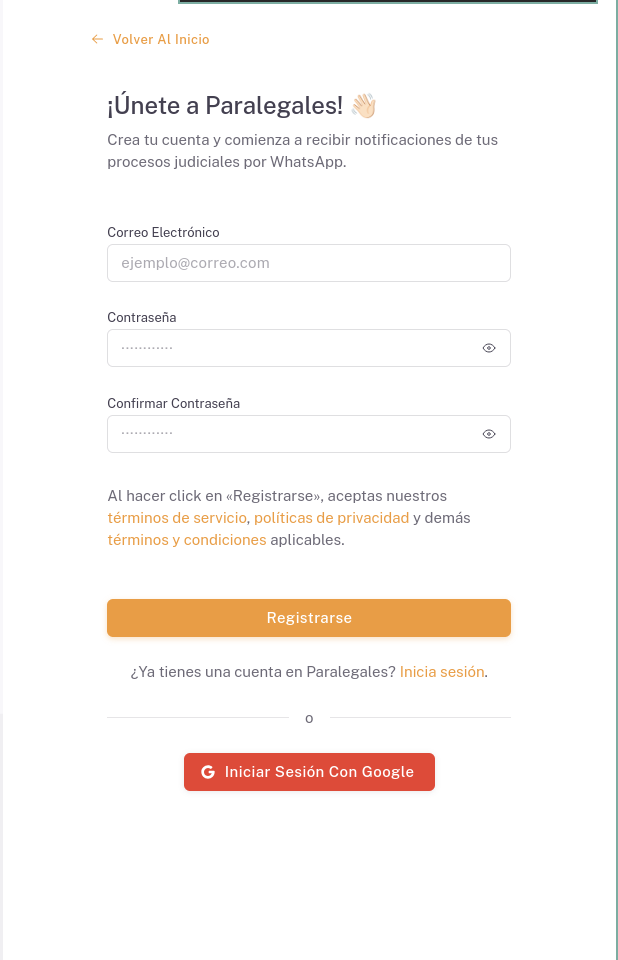
\includegraphics[width=0.85\textwidth]{img/figures/fig16-register.png}
  \caption[\registerScreenCaption]{\registerScreenCaption Fuente: Elaboración propia.}
  \label{fig:register-screen}
\end{figure}

\newcommand\ssoGoogleCaption{Flujo de autenticación mediante inicio de sesión único (SSO) con Google. \hspace{1em}}
\begin{figure}[H]
  \centering
  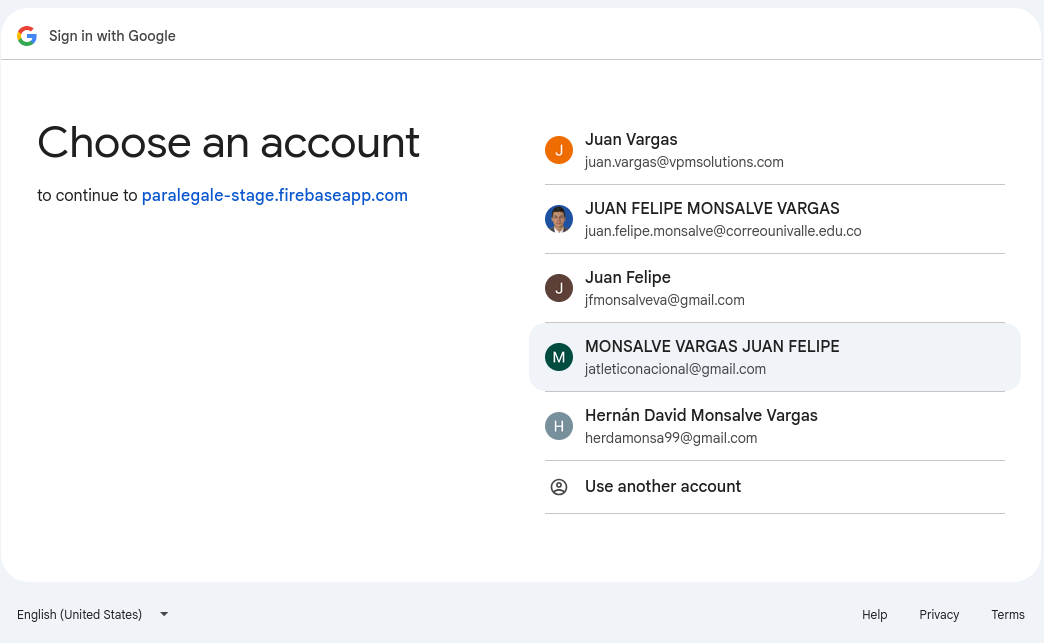
\includegraphics[width=1\textwidth]{img/figures/fig17-sso-google.png}
  \caption[\ssoGoogleCaption]{\ssoGoogleCaption Fuente: Elaboración propia.}
  \label{fig:sso-google}
\end{figure}

\begin{itemize}
  \item \textbf{Verificación de identidad por correo electrónico:} como política de seguridad para prevenir la proliferación de cuentas fraudulentas, se estableció como requisito obligatorio la validación de las direcciones de correo electrónico antes de habilitar el acceso total a la plataforma.

  \item \textbf{Recuperación de contraseña:} se incorporó un mecanismo seguro para el restablecimiento de credenciales de acceso. En caso de olvido, el usuario puede solicitar un enlace de recuperación enviado a su correo electrónico verificado, permitiendo retomar el control de la cuenta de manera autónoma y segura sin requerir intervención administrativa.
\end{itemize}

El proceso de verificación de identidad consta de dos pasos complementarios que se ilustran en las figuras \autoref{fig:email-verification-step} y \autoref{fig:email-verification-email}. En primer lugar, la plataforma informa al usuario sobre el requisito de validación y lo invita a revisar su bandeja de entrada; a continuación, el sistema envía un correo electrónico con el enlace de confirmación, bloqueando el acceso completo hasta que dicha acción sea completada.

\newcommand\emailVerificationStepCaption{Pantalla informativa del proceso de verificación de correo electrónico. \hspace{1em}}
\begin{figure}[H]
  \centering
  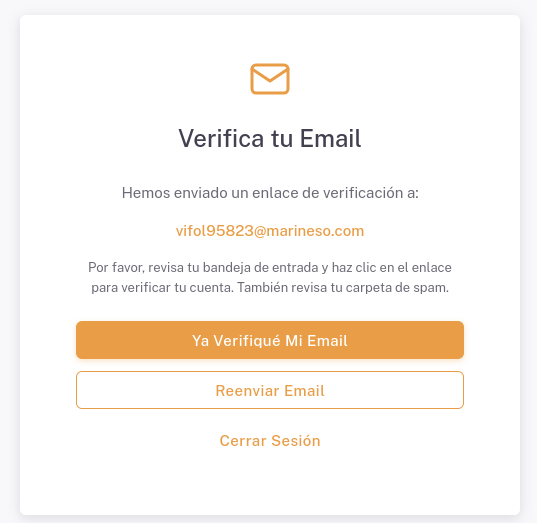
\includegraphics[width=0.85\textwidth]{img/figures/fig18-email-verification-step.png}
  \caption[\emailVerificationStepCaption]{\emailVerificationStepCaption Fuente: Elaboración propia.}
  \label{fig:email-verification-step}
\end{figure}

\newcommand\emailVerificationEmailCaption{Correo electrónico de verificación de identidad enviado al usuario tras el registro. \hspace{1em}}
\begin{figure}[H]
  \centering
  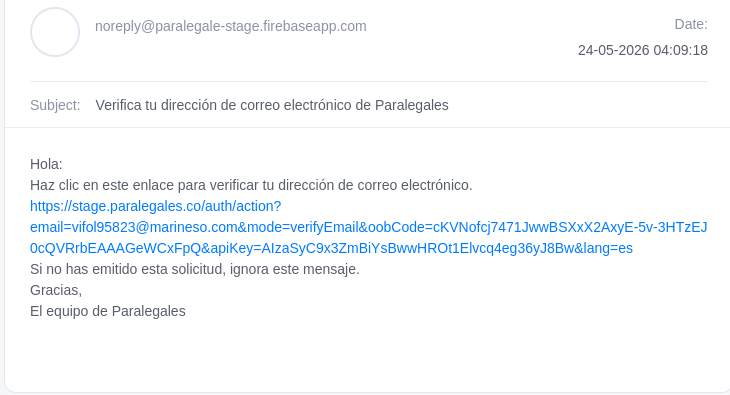
\includegraphics[width=0.65\textwidth]{img/figures/fig19-email-verification-email.png}
  \caption[\emailVerificationEmailCaption]{\emailVerificationEmailCaption Fuente: Elaboración propia.}
  \label{fig:email-verification-email}
\end{figure}

\begin{itemize}
  \item \textbf{Gestión y actualización de seguridad:} desde el panel de preferencias del perfil, los usuarios pueden gestionar directamente la seguridad de su cuenta. Se desarrollaron funcionalidades específicas para la actualización del correo electrónico y la modificación de contraseñas. Estas operaciones incorporan validaciones adicionales de protección, como la exigencia de la contraseña actual para confirmar cambios críticos, al tiempo que el sistema identifica y maneja inteligentemente el estado de los usuarios autenticados vía proveedores externos (SSO), adaptando la interfaz según corresponda.
\end{itemize}

Como se observa en la \autoref{fig:update-email-password}, la vista de seguridad del perfil unifica en una sola pantalla las opciones de actualización de correo y contraseña, adaptando su presentación según el proveedor de autenticación del usuario: los registros por SSO omiten los campos de contraseña, dado que la gestión de credenciales recae exclusivamente en el proveedor externo.

\newcommand\updateEmailPasswordCaption{Vista de gestión de seguridad de la cuenta con opciones de actualización de correo y contraseña. \hspace{1em}}
\begin{figure}[H]
  \centering
  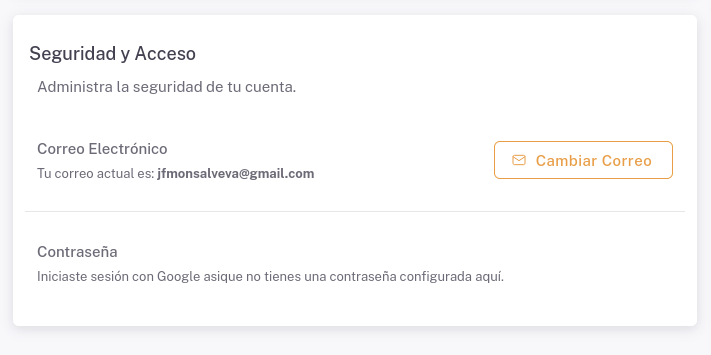
\includegraphics[width=1\textwidth]{img/figures/fig21-update-email-password-feature.png}
  \caption[\updateEmailPasswordCaption]{\updateEmailPasswordCaption Fuente: Elaboración propia.}
  \label{fig:update-email-password}
\end{figure}

\subsubsection{Interfaz Gráfica, Experiencia de Usuario y Onboarding}

El diseño visual del módulo se fundamenta en interfaces dinámicas que se adaptan al contexto del usuario. En lugar de crear vistas aisladas para cada flujo, se desarrolló un sistema de enrutamiento y componentes que consolida los diversos formularios en entornos visuales cohesivos, optimizando la navegación y reduciendo la carga cognitiva. Todo el proceso está acompañado por un manejo global de excepciones y mensajes de retroalimentación que guían al usuario de manera oportuna ante eventualidades, como interrupciones de red o uso de credenciales incorrectas.

Con el objetivo de enriquecer y personalizar la experiencia desde el primer ingreso a la plataforma, se diseñó e implementó un flujo de inicialización progresiva (\textit{onboarding}). Tras un registro exitoso, el sistema despliega una encuesta dinámica orientada a la perfilación del usuario, capturando datos profesionales relevantes tales como su nivel de especialidad legal, su profesión base y sus años de experiencia. Esta estructura de datos se somete a validación de esquemas en el entorno cliente para luego sincronizarse de manera inmediata con Firestore, lo que permite a la aplicación adaptar su funcionalidad a las necesidades particulares de cada cuenta. La \autoref{fig:onboarding} presenta el flujo de encuesta implementado, donde cada paso conduce al usuario a través de preguntas progresivas hasta completar su perfil inicial.

\newcommand\onboardingCaption{Flujo de \textit{onboarding} para la perfilación del usuario tras el registro. \hspace{1em}}
\begin{figure}[H]
  \centering
  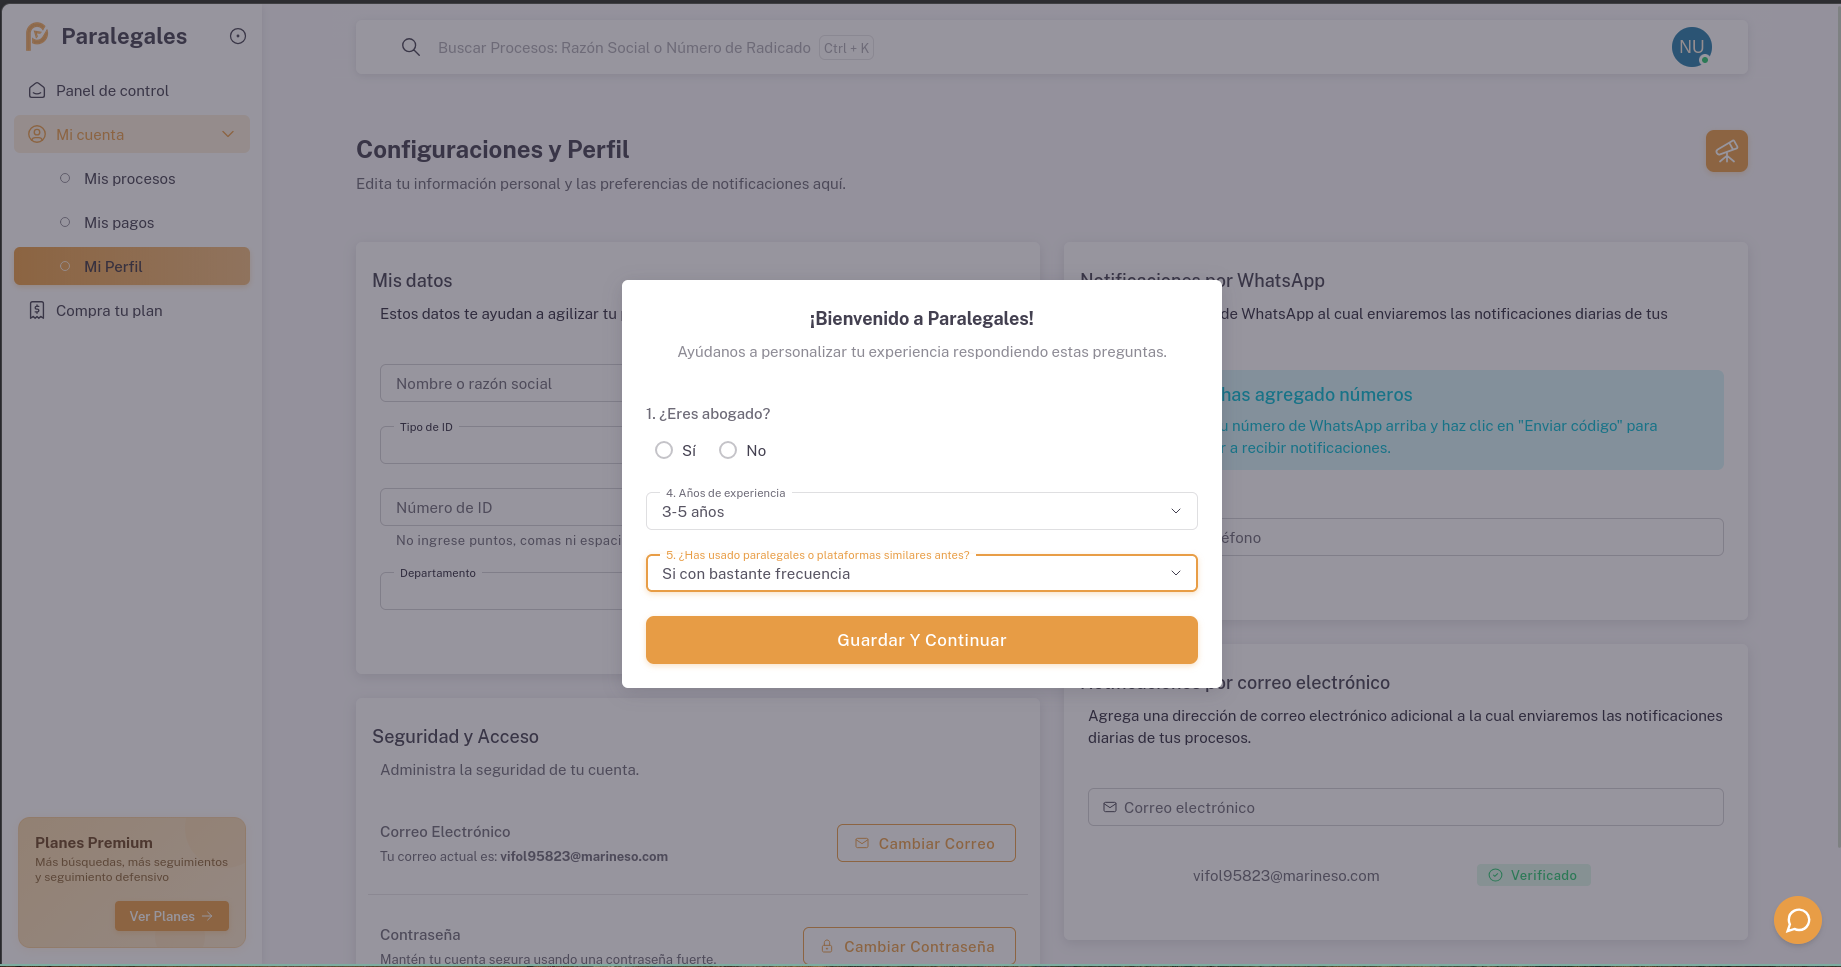
\includegraphics[width=1\textwidth]{img/figures/fig20-onboarding.png}
  \caption[\onboardingCaption]{\onboardingCaption Fuente: Elaboración propia.}
  \label{fig:onboarding}
\end{figure}

\subsubsection{Reglas de Seguridad y Control de Acceso a la Base de Datos}

De manera complementaria a la autenticación en el entorno cliente, se diseñaron e implementaron las Reglas de Seguridad de Firestore. Estas reglas son políticas declarativas que se evalúan y ejecutan directamente en los servidores de la base de datos antes de permitir cualquier operación de lectura o escritura, constituyendo la última y más robusta línea de defensa contra accesos no autorizados. Su implementación garantiza que los usuarios únicamente puedan interactuar con la información que les pertenece o sobre la que tienen permisos explícitos.

Dado que el control de acceso a los documentos representa una de las partes más críticas del sistema, el diseño de estas reglas estuvo respaldado por una batería de pruebas unitarias automatizadas. La inclusión de estos \textit{tests} permitió verificar de forma rigurosa cada política de acceso frente a múltiples escenarios y simulaciones de ataque, asegurando que ninguna brecha de seguridad comprometiera la privacidad ni la integridad de la información almacenada. La \autoref{fig:security-rules-firebase} ilustra el conjunto de reglas de seguridad implementadas sobre las colecciones principales de Firestore, donde cada documento está protegido mediante condiciones explícitas que validan la identidad del solicitante antes de autorizar cualquier operación. Una vez garantizado el control de identidad como cimiento transversal del sistema, el siguiente módulo entrega el valor central de la plataforma: la consulta, el seguimiento y la gestión de procesos judiciales.

\newcommand\securityRulesFirebaseCaption{Reglas de seguridad de Firestore que controlan el acceso a las colecciones de la plataforma. \hspace{1em}}
\begin{figure}[H]
  \centering
  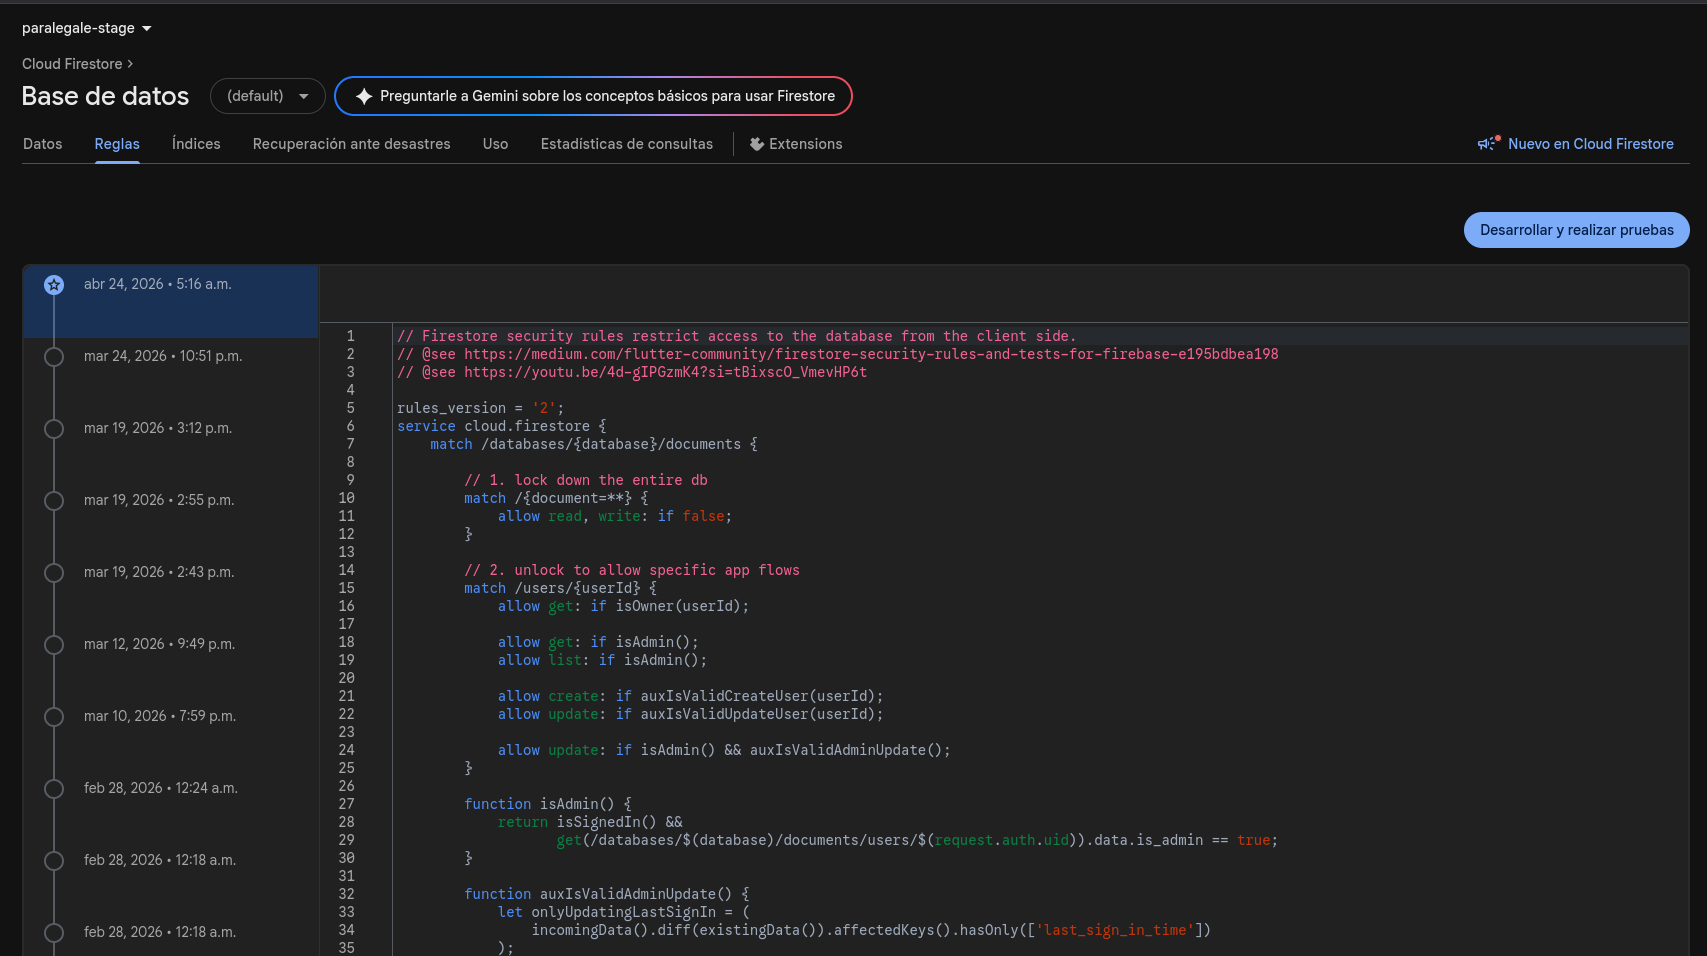
\includegraphics[width=1\textwidth]{img/figures/fig22-security-rules-in-firebase.png}
  \caption[\securityRulesFirebaseCaption]{\securityRulesFirebaseCaption Fuente: Elaboración propia.}
  \label{fig:security-rules-firebase}
\end{figure}
